
\documentclass[8pt]{beamer}

\geometry{paperwidth=168mm, paperheight=126mm}
\makeatletter
\newcommand*{\overlaynumber}{\number\beamer@slideinframe}
\makeatother
\mode<presentation> {

%\usetheme{CambridgeUS}
%\usetheme{Madrid}
%\usetheme{Frankfurt}
\usetheme{cern}

% As well as themes, the Beamer class has a number of color themes
% for any slide theme. Uncomment each of these in turn to see how it
% changes the colors of your current slide theme.

%\usecolortheme{beaver}
%\usecolortheme{dolphin}
%\usecolortheme{rose}
%\usecolortheme{whale}

%\setbeamertemplate{footline} % To remove the footer line in all slides uncomment this line
%\setbeamertemplate{footline}[page number] % To replace the footer line in all slides with a simple slide count uncomment this line

\setbeamertemplate{navigation symbols}{} % To remove the navigation symbols from the bottom of all slides uncomment this line
}

\usepackage{animate}
\usepackage{graphicx} % Allows including images
\usepackage{booktabs} % Allows the use of \toprule, \midrule and \bottomrule in tables

% Added by me
\usepackage[backend=bibtex,style=numeric,natbib=true, sorting=none]{biblatex}
\addbibresource{references.bib}
%\AtEveryCitekey{\iffootnote{\color{red}\tiny}{\color{blue}}}
\usepackage[absolute, overlay]{textpos}
\usepackage{xcolor}
\usepackage{multicol}
\usepackage{listings}
\usepackage{subcaption}
\usepackage{tabularx}
\usepackage{listings}
\usepackage[overlay,absolute]{textpos}
%\usepackage{parcolumns}
%\usepackage{enumitem}
\usepackage[font=scriptsize]{caption}
%\usepackage{libertine}
%\definecolor{light sky blue}{HTML}{82CAFA}
%\setbeamercolor{frametitle}{fg=blue!80!black}
\newcommand{\code}[1]{\texttt{#1}}
%\setbeamertemplate{bibliography item}{[\theenumiv]}
\setbeamertemplate{caption}[numbered]
\newcommand{\highr}{\textsuperscript{\textregistered}}
\defbeamertemplate{description item}{align left}{\insertdescriptionitem\hfill}


%%\newlength{\logowd}
%\setlength{\logowd}{14.046mm * \ratio{128mm}{254mm}}
%
%%\newlength{\logolw}
%\setlength{\logolw}{\footlinedp - 2.392mm * \ratio{128mm}{254mm}}
%
%%\newlength{\footlinetextwd}
%\setlength{\footlinetextwd}{140pt}
%
%%\newlength{\numberwd}
%\setlength{\numberwd}{20pt}

\pgfdeclareimage[width=1.2\logowd]{smalllogo}{cern-logo}
\pgfdeclareimage[width=1.2\logowd]{ntualogo}{ntua-logo}
%\pgfdeclareimage[width=\logowd]{mlablogo}{mlab-logo}

\setbeamertemplate{footline}
{
	\begin{beamercolorbox}[wd=\paperwidth,dp=\footlinedp,ht=1.2\footlineht,
		leftskip=\footlinesk,
		rightskip=\footlinesk]{footline}%
		\usebeamerfont{title in head/foot}%
		\lower\logolw\hbox{\pgfuseimage{ntualogo}}%
		\hspace{0.01cm}
%		\lower\logolw\hbox{\pgfuseimage{mlablogo}}%
%		\hspace{0.01cm}
		\lower\logolw\hbox{\pgfuseimage{smalllogo}}%
%		\hspace{-0.5cm}
		\makebox[\footlinetextwd][c]{\fontsize{10}{12}\selectfont \insertshortauthor}
		\hspace{-1.5cm}
		\makebox[\footlinetextwd][c]{\fontsize{10}{12}\selectfont \insertshortdate}%
		\hspace{-1.5cm}
		\makebox[\footlinetextwd][c]{\fontsize{10}{12}\selectfont \insertshorttitle}%
%		\hspace{-1cm}
		\hfill
		\makebox[\numberwd][r]{\fontsize{10}{12}\selectfont \insertframenumber}%
		\hspace{1cm}	
\end{beamercolorbox}%
}

%\setbeamerfont{footline}{size=\fontsize{12}{14}\selectfont}

%----------------------------------------------------------------------------------------
%	TITLE PAGE
%----------------------------------------------------------------------------------------

\title[HPC @ CERN]{Accelerating the World's Largest Accelerators} % The short title appears at the bottom of every slide, the full title is only on the title page
\subtitle{International HPC Summer School on HPC Challenges in Computational Sciences, Boulder, Colorado US}
\author{Konstantinos ILIAKIS} % Your name
\institute{CERN/NTUA} % Your institution as it will appear on the bottom of every slide, may be shorthand to save space

\date{\today} % Date, can be changed to a custom date

\begin{document}

\begin{frame}
\titlepage % Print the title page as the first slide
\end{frame}

%\begin{frame}
%\frametitle{Table of Contents} % Table of contents slide, comment this block out to remove it
%\tableofcontents
%\tableofcontents[pausesections] % Throughout your presentation, if you choose to use \section{} and \subsection{} commands, these will automatically be printed on this slide as an overview of your presentation
%\end{frame}

%----------------------------------------------------------------------------------------
%	PRESENTATION SLIDES
%----------------------------------------------------------------------------------------



\begin{frame}
	\frametitle{Abstract}
	\begin{itemize}
		\item CERN -- European Organization for Nuclear Research
		\item Doctoral Student with NTUA as supervising university
		\item Computer architecture and hard/soft-ware HPC techniques to 
		accelerate complex simulators
	\end{itemize}
	% What is CERN
	% What I am doing at CERN
	% Thesis abstract
\end{frame}


\begin{frame}
	\frametitle{BLonD (I)}
	\begin{textblock}{2}(5,0)
		\begin{figure}
			
\includegraphics[width=\textwidth]{figures/BLonD_logo_header}
		\end{figure}
	\end{textblock}
	\begin{itemize}
		\item \underline{B}eam \underline{Lon}gitudinal \underline{D}ynamics code simulator
		\item Developed in Python with C extensions for the computational kernels
		\item More than ten contributors, numerous users at CERN and KEK-Japan
	\end{itemize}
	% What is blond
	% what research has been conducted with blond, 
	% current users, publications
\end{frame}

\begin{frame}
%	\frametitle{Blond II}
		\begin{columns}[t]
			\column{0.7\textwidth}\centering
			LHC Blow-up\\
			\begin{figure}[h]
				\hspace{-12pt}
				\animategraphics[loop,autoplay, height=.46\textheight] {10} {figures/LHC_Blow-up/LHC_Blow-up-}{0}{0} %89
				\caption*{Insert caption}
			\end{figure}
			
			\column{0.46\textwidth}\centering
%			\vspace{-25pt}
			PS-SPS Transfer\\
			\begin{figure}[h]
				\animategraphics[loop,autoplay,height=.48\textheight] {8} {figures/PS-SPS_Transfer/PS-SPS_Transfer-}{0}{0} %104
				\caption*{Insert caption}
			\end{figure}
		\end{columns}
\end{frame}


\begin{frame}
	\frametitle{BLonD++}
	% What is blond++, facts and numbers
	% benchmark comparison with blond
	{ \small
	\begin{itemize}
		\item BLonD++ is the C++ version of BLonD
		\item Native support for multi-threading, auto-vectorization, compiler optimizations etc
		\item Proved to perform better in complex simulations
	\end{itemize}
	}
%	\vspace{-10pt}
	\begin{figure}
		\hspace{-150pt}	
		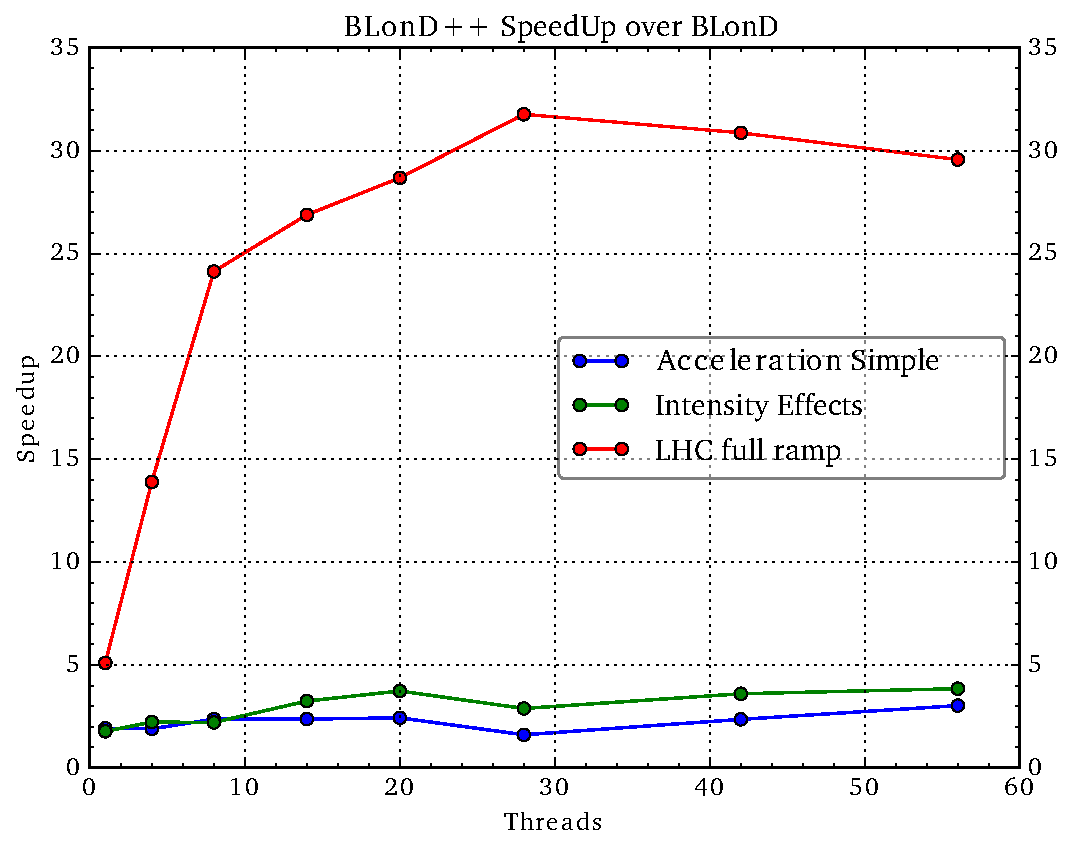
\includegraphics[width=.5\textwidth]{figures/BLonDpp-speedup2}
	\end{figure}
\end{frame}

\begin{frame}
	\frametitle{Future Studies}
	% Future challenges + plans
\end{frame}


%The Beam Longitudinal Dynamics code BLonD is a unique simulation code developed at CERN in the BE-RF group to model beam motion in synchrotrons. Beam parameters for important upgrades and future studies are based on the results of BLonD simulations. The code is written in a modular fashion, so that the physics content of each simulation can be adapted to special purposes via modules pipelining. The code was originally developed in python and has been now translated to C++ to apply various optimization techniques. The present CERN grid infrastructure restricts the complexity of physics problems that can be modelled due to performance limitations. A dedicated computer architecture is necessary to meet the present and growing future computational needs in the field of longitudinal beam dynamics.

%Given these needs, studying computer architectures and hardware accelerators suitable specifically for complex simulators is essential. The interaction between different modules has to be investigated in detail. Selecting a few representative, physics cases, the feasibility and performance of different combinations of architecture including Xeon Phi, GPU, and FPGA components are to be evaluated. In the first stage, testing on the existing CERN OpenLab and TechLab infrastructures is envisaged. Eventually, prototype hardware acquisition for testing purposes is likely to be necessary. Ideally, the outcome of the PhD thesis will be a proposal for a concrete, dedicated computer architecture that will be purchased and used for longitudinal beam dynamics studies.


%\begin{frame}{LHC\_Blow-up animation}
%\animategraphics[loop,autoplay,width=\linewidth]{10}{figures/LHC_Blow-up/LHC_Blow-up-}{0}{89}
%\end{frame}
%
%\begin{frame}{PS-SPS\_Transfer animation}
%\animategraphics[loop,autoplay,height=.8\textheight]{8}{figures/PS-SPS_Transfer/PS-SPS_Transfer-}{0}{104}
%\end{frame}


%%------------------------------------------------
%%\section{Introduction} % Sections can be created in order to organize your presentation into discrete blocks, all sections and subsections are automatically printed in the table of contents as an overview of the talk
%%------------------------------------------------
%
%%\setlength{\columnsep}{0.6cm}
%\definecolor{background}{rgb}{0.95, 0.95, 0.92}
%\definecolor{mygreen}{rgb}{0, 0.6, 0}
%
%\lstdefinestyle{mystyle}{
%	backgroundcolor=\color{background},
%	%	breaklines=true,
%	commentstyle=\color{mygreen},
%%	numbers=left,
%%	numbersep=5pt,
%	frame=single,
%	tabsize=3
%}
%\lstset{style=mystyle, aboveskip=10pt, basicstyle=\tiny}
%
%\subsection{The MapReduce Programming Model}
%\renewcommand{\footnotesize}{\tiny}
%
%%\subsection{MapReduce in Shared-Memory Systems}
%\begin{frame}[t, fragile]
%	\frametitle{MapReduce in Distributed Systems (\RN{\overlaynumber})}
%	\begin{itemize}
%		\item MapReduce was originally proposed by Google \footfullcite{dean2008mapreduce} and later open-sourced by Apache Hadoop \footfullcite{hadoop2009hadoop}. 
%		\item Enabled automatic parallelization of functional programs.
%		\item The runtime handles the tasks of fault tolerance, dynamic scheduling, data partitioning and communication.
%		\item Huge success in large scale distributed computation. 
%	\end{itemize}
%\vspace{-17pt}
%\begin{multicols}{2}
%
%\begin{onlyenv}<2->
%\begin{minipage}{0.45\textwidth}
%	\begin{lstlisting}[language=C, title={Map function of Word Count}, captionpos=b]
%void map(string key, string value){
%	// key: document name
%	// value: the text of the document
%	for(each word in value){
%		emit_intermediate(word, 1);
%	}
%}
%	\end{lstlisting}
%\end{minipage}
%\end{onlyenv}
%
%\columnbreak
%
%\begin{onlyenv}<3->
%\begin{minipage}{0.48\textwidth}
%	\begin{lstlisting}[language=C, title={Reduce function of Word Count}, captionpos=b]
%void reduce(string key, int values[]){
%	// key: a word
%	// values[]: an array of numbers
%	int result = 0;
%	for(each value in values){
%		result += value;
%	}
%	emit_out(result);
%}
%	\end{lstlisting}
%	\vspace{-10pt}
%\end{minipage}
%\end{onlyenv}
%\end{multicols}
%\end{frame}
%
%
%\begin{frame}
%	\frametitle{MapReduce with Shared-Memory Properties}
%	\begin{itemize}
%		\item Modern high performance processors and accelerators \footfullcite{chrysos2014intel},\footfullcite{lindholm2008nvidia} integrate hundreds to thousands cores in a single chip.
%		\item They exhibit similarities with clustered systems.
%		\item Many parallel programming frameworks have emerged. However, coding efficient parallel programs is still tedious.
%		\item Phoenix \footfullcite{ranger2007evaluating} and Metis \footfullcite{mao2010optimizing} are frameworks that adjust MapReduce to the needs of shared-memory processors.
%	\end{itemize}
%\end{frame}
%
%\begin{frame}
%	\frametitle{Shared-Memory MapReduce Applicability}
%	\vspace{-10pt}
%	\begin{figure}[h]
%		\includegraphics[width=0.5\textwidth]{../Figures/mr_vs_pthreads.pdf}
%		\caption*{Phoenix++ \footfullcite{talbot2011phoenix++} vs Pthreads implementation in a 56-core multi-processor. The speedup is with respect to the same sequential code \footfullcite{ranger2007evaluating}.}
%	\end{figure}
%	\vspace{-15pt}
%	\begin{itemize}
%		\item Comparable performance and scalability.
%		\item Automatic concurrency management, scheduling, parallelization.
%		\item Conclusion: MapReduce is a promising programming model for shared-memory systems.
%	\end{itemize}
%\end{frame}
%
%\begin{frame}
%	\frametitle{Traditional Phoenix Architecture}
%	\begin{columns}[c]
%	\column{0.7\textwidth}
%	\begin{figure}[h]
%		\hspace{-12pt}	
%%		\includegraphics[width=1.0\textwidth]{../Figures/tmr-1-top.pdf}
%		\caption*{Shared-Memory MapReduce Architecture	\footnotemark}
%%		\label{fig:phoenix-architecture}
%	\end{figure}
%	
%	\column{0.46\textwidth}
%%	\vspace{-25pt}
%	\begin{block}{Work flow}
%	\begin{enumerate}
%		\item Split input
%		\item Initialize map workers
%		\item Execute map tasks, emit in intermediate buffer
%		\item Execute reduce tasks, store results in final buffer
%		\item Merge\&Sort in parallel
%		\item Final results are in output buffer
%	\end{enumerate}
%	\end{block}
%	\end{columns}
%	\footnotetext{\fullcite{chen2010tiled}}
%\end{frame}
%
%\subsection{Proposal Overview}
%
%\begin{frame}
%	\frametitle{Traditional Work-flow Inefficiency}
%	\begin{onlyenv}<1>
%	\begin{figure}[h]
%		\begin{subfigure}{\textwidth}
%%			\includegraphics[width=1.0\textwidth]{../Figures/conventional-workflow.pdf}
%			\caption{Conventional Work-flow}
%		\end{subfigure}
%		\par\vspace{15pt}
%		\begin{subfigure}{\textwidth}
%%			\includegraphics[width=1.0\textwidth]{../Figures/pipelined-workflow-2.pdf}
%			\caption{Decoupled Work-flow}
%		\end{subfigure}
%	\end{figure}
%	\end{onlyenv}
%	\begin{onlyenv}<2>
%		
%	\begin{figure}[h]
%			\centering
%%			\includegraphics[width=.5\textwidth]{../Figures/untitled.pdf}
%			\caption*{Task scheduling comparison}
%	\end{figure}
%	\end{onlyenv}
%	\begin{block}{Decoupled Map-Combine}
%		\begin{itemize}
%			\item Map and Combine are fully decoupled and overlapped.
%			\item Efficient resource utilization.
%			\item Profit from pipeline parallelism.
%		\end{itemize}
%	\end{block}
%\end{frame}
%
%
%
%
%\begin{frame}
%	\frametitle{Proposal Description and Rest Contributions}
%	\centerline{\textbf{Pipelined MapReduce}}
%	\begin{itemize}
%		\item We decouple Map and Combine into two separate phases.
%		\item We introduce a high-performance, concurrent queue to pipeline data from Map to Combine tasks
%		\item We develop a communication pattern aware, thread-to-CPU binding policy to minimize queue manipulation overheads.
%		\item We add batched consumes functionality to further improve queue performance.
%		\item We attempt to characterize the suitability of different applications to our architecture, based on metrics derived from hardware counters \footfullcite{intelvtune1}, \footfullcite{eventshswell}.
%	\end{itemize}
%\end{frame}
%%------------------------------------------------
%%------------------------------------------------
%\section{Implementation Details}
%%------------------------------------------------
%
%
%
%\subsection{Pipelined MapReduce Architecture}
%%\begin{frame}
%%	\frametitle{Pipelined MapReduce Architecture}
%%	\begin{columns}[c]
%%		\column{0.73\textwidth}
%%		\begin{figure}[h]
%%			\includegraphics[width=\textwidth]{../Figures/pipelined-arch-top.pdf}
%%			\label{fig:pipelined-mr-arch}
%%		\end{figure}
%%		
%%		\column{0.42\textwidth}
%%		\begin{block}{Deviations from the traditional scheme}
%%		\begin{enumerate}
%%			\item Two thread pools
%%			\item Execute map tasks, pipeline intermediate data to combiners
%%			\item Concurrently read the data, combine and emit in local containers
%%		\end{enumerate}
%%		\end{block}
%%	\end{columns}
%%\end{frame}
%
%\begin{frame}
%	\frametitle{Pipelined MapReduce Architecture}
%		\vspace{-10pt}
%		\begin{figure}[h]
%			%		\centering
%%			\includegraphics[width=.9\textwidth]{../Figures/pipelined-arch-top.pdf}
%			%\caption[Batch Size Effect on Xeon Phi]{Batch Size Effect on Xeon Phi}
%			\label{fig:pipelined-mr-arch}
%		\end{figure}
%		
%		\vspace{-7pt}
%		\begin{block}{Deviations from the traditional scheme}
%			\begin{enumerate}
%				\item Two thread pools
%				%			\item Bind threads to CPUs, considering their communication pattern
%				\item Execute map tasks, pipeline intermediate data to combiners
%				\item Concurrently read, combine and emit in local containers
%			\end{enumerate}
%		\end{block}
%\end{frame}
%
%\subsubsection*{Concurrent Shared Buffer}
%\begin{frame}
%	\frametitle{High Performance Shared Buffer Implementation}
%	\begin{columns}[c]
%	\column{0.82\textwidth}
%%	\vspace{-1cm}
%	\begin{figure}[h]
%		\begin{subfigure}{0.49\textwidth}
%%			\centering
%%			\includegraphics[width=\textwidth]{../Figures/bench-queues/haswell/concurrent.pdf}
%			\label{fig:bench-queue-haswell-concurrent}
%			\caption*{Haswell}
%		\end{subfigure}
%%	\end{figure}
%%	\vspace{-20pt}
%%	\begin{figure}[h]
%		\begin{subfigure}{0.49\textwidth}
%%		\hspace{-25pt}
%%			\centering
%%			\includegraphics[width=\textwidth]{../Figures/bench-queues/phi/concurrent.pdf}
%			\label{fig:bench-queue-phi-concurrent}
%			\caption*{Xeon Phi}
%	\end{subfigure}
%	\end{figure}
%
%	\column{.33\textwidth}
%	Benchmarked queues:\small{\begin{enumerate}
%		\item Boost-Dynamic \footnotemark
%		\item Boost-Static
%		\item Cameron \footnotemark
%		\item Circuclar FIFO \footnotemark 
%		\item Folly SPSC \footnotemark
%	\end{enumerate}}
%	Based on performance, but also API, we decided to use Boost's SPSC queue, with static memory allocation.
%	\end{columns}
%	\footnotetext[12]{Tim Blechmann. \emph{boost::lockfree::spsc\_queue}}
%	\footnotetext[13]{Cameron. \emph{A Fast Lock-Free Queue for C++}}
%	\footnotetext[14]{Kjell Kod. \emph{Lock-Free SPSC Queue.}}
%	\footnotetext[15]{Bo Hu and Jordan DeLong. \emph{folly::ProducerConsumerQueue}}
%\end{frame}
%
%
%\subsubsection*{Memory Aware Thread-to-CPU Binding Policies}
%\begin{frame}[t]
%	\frametitle{Communication Aware Thead-to-CPU Binding Policies (\RN{\overlaynumber})}
%	\begin{columns}[t] % The "c" option specifies centered vertical alignment while the "t" option is used for top vertical alignment
%	\column{.65\textwidth} % Left column and width
%	\vspace{-25pt}
%	
%	\begin{figure}[h]
%%	\par\hspace{-30pt}
%		\begin{onlyenv}<1->
%		
%		\begin{subfigure}{1.\textwidth}
%%			\includegraphics[width=\textwidth]{../Figures/thread-to-cpu-policies/thread-to-cpu-policy-1-crop.pdf}
%			\label{fig:policy-dedicated}
%		\end{subfigure}
%		\end{onlyenv}
%%	\par\hspace{-30pt}
%		%	\hspace{10pt}
%%	\par\hspace{-27pt}	
%		%	\par\vspace{10pt}
%		\begin{onlyenv}<2->
%			
%		
%		\begin{subfigure}{1.\textwidth}
%%			\includegraphics[width=\textwidth]{../Figures/thread-to-cpu-policies/thread-to-cpu-policy-3-crop.pdf}
%			\label{fig:policy-push}
%		\end{subfigure}
%		\end{onlyenv}
%		
%		\begin{onlyenv}<3->
%		\begin{subfigure}{1.\textwidth}
%%			\includegraphics[width=\textwidth]{../Figures/thread-to-cpu-policies/thread-to-cpu-policy-2-crop.pdf}
%			\label{fig:policy-fill}
%		\end{subfigure}
%		\end{onlyenv}
%		
%		\label{fig:thread-to-cpu-policies}
%	\end{figure}
%%	\par\hspace*{-1cm}
%	\column{.45\textwidth} % Right column and width
%%	\par\hspace{-40pt}
%	\vspace{-20pt}
%	\begin{block}{Dedicated}<1->
%		First cores are allocated by mappers, last by combiners.
%	\end{block}
%	\vspace{10pt}
%	\begin{block}{Push}<2->
%		Bind one mapper per core, then bind combiners on top.
%	\end{block}
%	\vspace{12pt}
%	\begin{block}{Fill}<3->
%		Map and Combine threads are interleaved to minimize their distance.
%	\end{block}
%%	\begin{block}{Policies}
%%	\begin{itemize}
%%	\item<1-> Dedicated: First cores are used for mappers, last for combiners.
%%	\item<2-> Push: Bind one mapper per core, then bind combiners on top.
%%	\item<3-> Fill: Map and Combine threads are interleaved to minimize their distance.
%%	\end{itemize}
%%	\end{block}
%	\end{columns}
%
%\end{frame}
%
%%\subsubsection*{Framework Modularity}
%%\begin{frame}
%%	\frametitle{Tunable Variables for Top Performance}
%%	\begin{columns}[c]
%%	
%%	\column{0.8\textwidth}
%%%	\begin{table}
%%%		\resizebox{0.8\textwidth}{!}{
%%%			\begin{tabular}{|l|p{0.3\linewidth}|p{0.25\linewidth}|}
%%%				\specialrule{.1em}{0.00em}{.00em}
%%%				\textbf{Variable name} & \textbf{Description} & \textbf{Default Value} \\
%%%				
%%%				\specialrule{.1em}{0.00em}{.00em}
%%%				MR\_NUMTHREADS & Number of Threads & Number of logical cores \\
%%%				\hline
%%%				
%%%				MR\_NUMMAPTASKS & Number of Map Tasks & $ map\_threads \times 16 $ \\
%%%				\hline
%%%				
%%%				MR\_NUMREDUCETASKS & Number of Reduce Tasks & Number of Map threads\\
%%%				\hline
%%%				
%%%				MR\_CHUNKSIZE & Multiplier of Task size & 1 \\
%%%				\hline		
%%%			\end{tabular}
%%%			
%%%		}
%%%	\end{table}
%%%	\vspace{-10pt}
%%	
%%	\begin{table}
%%%		\hspace{-10pt}
%%		\resizebox{.8\textwidth}{!}{
%%%			\renewcommand{\arraystretch}{1.5}
%%%			\renewcommand{\tabcolsep}{0.2cm}
%%			\begin{tabular}{|l|p{0.3\linewidth}|p{0.25\linewidth}|}
%%				\specialrule{.1em}{0.00em}{.00em}
%%				\textbf{Variable name} & \textbf{Description} & \textbf{Default Value} \\
%%				
%%				\specialrule{.1em}{0.00em}{.00em}
%%				
%%				MR\_CHUNKSIZE & Multiplier of Task size & 1 \\
%%				\hline
%%				
%%				MR\_MAP\_COMBINE\_RATIO & Mappers / Combiners ratio & 1 \\
%%				\hline
%%				
%%				MR\_THR\_TO\_CPU\_POLICY & Thread to CPU binding policy & 1 (Fill policy) \\
%%				\hline
%%				
%%				MR\_BUF\_SIZE & SPSC Queue fixed-size & 1000\\
%%				\hline
%%				
%%				MR\_BATCH\_SIZE & Read block size & 50 \\
%%				\hline
%%				
%%%				MR\_MAP\_SLEEP\_TIME & Full buffer sleep interval & 100 nano sec \\
%%%				\hline	
%%			\end{tabular}
%%		}
%%				     
%%		%		\caption{MapReduce Runtime Configurable Variables}
%%	\end{table}
%%	
%%	\column{0.33\textwidth}
%%	\begin{block}{Top Array}
%%	MapReduce runtime configurable variables
%%	\end{block}
%%%	\begin{block}{Bottom Array}
%%%	Pipeline and Queue specific variables
%%%	\end{block}
%%\end{columns}
%%\end{frame}
%
%\subsection{Other Contributions}
%\subsubsection*{Synthetic Test Suite}
%\begin{frame}
%	\frametitle{Synthetic Test Suite}
%	\begin{columns}[t]
%	\column{0.65\textwidth}
%	\vspace{-20pt}
%	\begin{figure}[h]
%%		\centering
%%		\includegraphics[scale=0.4]{../Figures/dummy2cpu-mem-v2.pdf}
%		\caption*{Test case with compute intensive map phase and memory intensive combine phase.}
%	\end{figure}
%	
%	\column{0.4\textwidth}
%	\vspace{-20pt}
%	\begin{block}{Usefulness}
%	We used it to imitate combinations of different workload types of adjustable heaviness.\\[5pt]
%	Trigonometric and exponential functions are used for CPU-bound workloads. Pseudo-random memory access in wide arrays is used for memory-bound workloads.
%%	Helped us benchmark and further understand the behavior of our architecture.\\[5pt]
%%	The figure demonstrates the dependency of optimal mappers/combiners ratio on map/combine workload weight distribution.
%	\end{block}
%	\end{columns}
%
%\end{frame}
%
%\subsubsection*{Benchmark Applications}
%\begin{frame}
%	\frametitle{Benchmark Applications \footfullcite{talbot2011phoenix++}}
%	\setbeamertemplate{description item}[align left]
%	\begin{description}
%		\item[Histogram] Generate the frequency histogram of 8-bit RGB pixel bitmap.
%		\item[KMeans] Iteratively group n-dimensional points into a user specified number of clusters, until convergence is reached.
%		\item[Linear Regression] Compute the line that best fits a set of coordinates.
%		\item[Matrix Multiply] Calculate the product of 2 equal-size, square matrices.
%		\item[PCA] Calculate mean and covariance vector of a set of points, as the first steps of Principal Component Analysis.
%		\item[Word Count] Count the frequency of each unique word in a text file.
%	\end{description}
%\end{frame}
%
%\subsubsection*{Application Characterization}
%\begin{frame}[t]
%	\frametitle{Application Characterization in Haswell (\RN{\overlaynumber})}
%%	\vspace{-25pt}
%	\centering\small{\begin{math}
%		IPB = \frac{Instructions}{Input\_Byte}\quad
%		MSPI = \frac{Memory\_Stalls}{Instruction}\quad
%		RSPI = \frac{Resource\_Stalls}{Instruction}
%		\end{math}}
%	\begin{columns}[t]
%		\column{0.5\textwidth}
%		\begin{onlyenv}<1->
%		
%		\begin{figure}
%%			\centering
%			\vspace{-15pt}
%%			\includegraphics[width=\textwidth]{../Figures/haswell/hardware-counters/original/default_containers.pdf}
%			\caption*{Phoenix++, Default Containers}
%			\label{fig:original-counters-normal}
%		\end{figure}
%		
%		\vspace{-20pt}
%		\scriptsize{\begin{itemize}
%			\item Hist and LR have very low complexity and rare stalls, thus bad candidates
%			\item KMeans and MM have sufficient complexity and stalls, thus suitable
%			\item WC and PCA are hard to tell
%		\end{itemize}}
%		
%		\end{onlyenv}	
%		
%		\column{0.5\textwidth}
%		\begin{onlyenv}<2->
%		
%		\begin{figure}
%			\vspace{-15pt}
%%			\includegraphics[width=\textwidth]{../Figures/haswell/hardware-counters/original/hash_containers.pdf}
%			\caption*{Phoenix++, Hash Containers}
%			\label{fig:original-counters-hash}
%		\end{figure}
%		\vspace{-20pt}
%		\scriptsize{\begin{itemize}
%			\item Generally increased complexity due to hash containers.
%			\item Hist and LR experience frequent stalls, more likely to be suitable.
%			\item KMeans, MM and WC are ideal candidates
%			\item PCA is again, hard to tell
%		\end{itemize}}
%		\end{onlyenv}			
%	\end{columns}
%\end{frame}
%%------------------------------------------------
%\section{Results}
%%------------------------------------------------
%
%\subsection{Experimental Setup}
%\begin{frame}
%	\frametitle{Experimental Setup Overview I}
%	\begin{columns}[c]
%		\column{0.5\textwidth}
%		\begin{block}{Intel\highr Xeon Phi\texttrademark{}}
%		\begin{itemize}
%			\item High performance Co-processor \footnotemark
%			\item Features 57 MIC in-order cores @ 1.1GHz
%			\item 4 Hardware threads per core
%			\item 256KB L2 cache
%			\item L2 memory controllers are inter-connected via a bidirectional ring
%		\end{itemize}
%		\end{block}
%		
%		\column{0.6\textwidth}
%		\begin{figure}
%%			\includegraphics[width=\textwidth]{../Figures/xeon_phi_arch.jpg}
%		\end{figure}
%		
%	\end{columns}
%	\footnotetext{\fullcite{jeffers2013intel}}
%\end{frame}
%
%
%\begin{frame}
%	\frametitle{Experimental Setup Overview II}
%	\begin{columns}[c]
%		\column{0.5\textwidth}
%		\begin{block}{Dual-Socket Intel\highr{} Haswell}
%			\begin{itemize}
%				\item 4th Generation Intel Micro-architecture \footnotemark
%				\item Two sockets, 64GB RAM in total
%				\item 14 cores @ 2GHz per socket 
%				\item 2 hardware threads per core
%				\item 256KB L2 cache per core
%				\item 35MB L3 cache per socket
%			\end{itemize}
%		\end{block}
%		\column{0.63\textwidth}
%		\begin{figure}
%%			\includegraphics[width=\textwidth]{../Figures/hsw_die_funct.jpg}
%		\end{figure}
%	\end{columns}
%	\footnotetext{\fullcite{hammarlund2014haswell}}
%\end{frame}
%
%
%\subsection{Optimizations Evaluation}
%%\subsubsection*{Static-Dynamic Queue Comparison}
%%\begin{frame}
%%	\frametitle{Boost with Static vs Dynamic Memory Allocation}
%%	\begin{columns}[t]
%%	\column{0.7\textwidth}
%%	\vspace{-25pt}
%%	\begin{figure}
%%		\includegraphics[scale=0.3]{../Figures/haswell/boost-dynamic-static-haswell.pdf}
%%		\caption*{Haswell}
%%	\end{figure}
%%	\vspace{-1cm}
%%	\begin{figure}
%%		\includegraphics[scale=0.3]{../Figures/phi/boost-dynamic-static-phi.pdf}
%%			\caption*{Xeon Phi}
%%	\end{figure}
%%
%%	\column{0.4\textwidth}
%%	\begin{block}{Static Memory Allocation}
%%	\begin{itemize}
%%		\item Enables various compiler optimizations
%%		\item 
%%	\end{itemize}
%%	\end{block}
%%	\end{columns}
%%
%%\end{frame}
%
%\subsubsection*{Thread-to-CPU Binding Policies Evaluation}
%\begin{frame}[t]
%	\frametitle{Memory-aware Thread-to-CPU Binding Policy Speedup (\RN{\overlaynumber})}
%	\begin{columns}[t]
%		\column{0.7\textwidth}
%		\vspace{-35pt}
%		\begin{onlyenv}<1->
%			
%		
%		\begin{figure}
%%			\includegraphics[width=.8\textwidth]{../Figures/haswell/policies-haswell.pdf}
%			\caption*{Haswell}
%		\end{figure}
%		\end{onlyenv}
%		\vspace{-1cm}
%		\begin{onlyenv}<2->
%		\begin{figure}
%			\includegraphics[width=.8\textwidth]{../Figures/phi/policies-phi.pdf}
%			\caption*{Xeon Phi}
%		\end{figure}
%		\end{onlyenv}
%		\column{0.44\textwidth}
%		\begin{block}{Haswell}<1->
%			Fill policy binds co-operating threads in the same socket $ \rightarrow $ speedup from NUMA-awareness
%		\end{block}
%		\begin{block}{Xeon Phi}<2->
%			All L2 caches are fully coherent and inter-connected. Single UMA node $ \rightarrow $ non-observable speedup
%		\end{block}
%%		Speedup of Fill policy over Dedicated and Push.
%	\end{columns}
%\end{frame}
%
%\subsubsection*{Batched Updates Evaluation}
%\begin{frame}[t]
%	\frametitle{Batched Reads Speedup (\RN{\overlaynumber})}
%	\begin{columns}[t]
%		\column{0.7\textwidth}
%		\vspace{-35pt}
%		\begin{onlyenv}<1->
%		\begin{figure}
%			\includegraphics[width=.8\textwidth]{../Figures/haswell/consume-one-batch-haswell.pdf}
%			\caption*{Haswell}
%		\end{figure}
%		\end{onlyenv}
%		\vspace{-1cm}
%		\begin{onlyenv}<2->
%		\begin{figure}
%			\includegraphics[width=.8\textwidth]{../Figures/phi/consume-one-batch-phi.pdf}
%			\caption*{Xeon Phi}
%		\end{figure}
%		\end{onlyenv}
%		\column{0.45\textwidth}
%		\begin{block}{\code{consume\_batch(\\Functor f, size\_t batch)}}<1->
%		\begin{itemize}
%			\item Based on boost's \code{consume\_all()}
%			\item Zero data copying
%			\item Reduces congestion on control variables
%			\item Improves cache locality
%			\item $ \approx $ 20--50 blocks per buffer for adequate performance 
%		\end{itemize}
%		\end{block}
%	\end{columns}
%\end{frame}
%
%\subsection{Performance Benchmark}
%\begin{frame}[t]
%	\frametitle{Pipelined MR VS Phoenix++ in Haswell (\RN{\overlaynumber})}
%	\begin{columns}[t]
%		\column{0.7\textwidth}
%		\vspace{-35pt}
%
%		\begin{onlyenv}<1->
%		\begin{figure}
%			\includegraphics[width=.8\textwidth]{../Figures/haswell/input-sizes-haswell-normal.pdf}
%			\caption*{Default Containers}
%		\end{figure}
%		\end{onlyenv}
%
%		\vspace{-1cm}
%
%		\begin{onlyenv}<2->
%		\begin{figure}
%			\includegraphics[width=.8\textwidth]{../Figures/haswell/input-sizes-haswell-hash.pdf}
%			\caption*{Hash Containers}
%		\end{figure}
%		\end{onlyenv}
%
%		
%		\column{0.45\textwidth}
%		\vspace{-25pt}
%		\scriptsize{\begin{block}<1->{Default Containers}
%		\begin{itemize}
%			\item KMeans and MM improved
%			\item Hist and LR slowed down
%			\item PCA and WC similar
%%			\item Good agreement with predicted suitability
%		\end{itemize}
%		\end{block}}
%		\scriptsize{\begin{block}<2->{Hash Containers}
%		\begin{itemize}
%			\item Hist, KMeans, LR, MM and WC improved
%			\item PCA 20.4\% average slow-down
%%			\item Good agreement with predicted suitability
%			\item Resource saturation in large input
%		\end{itemize}
%		\end{block}}
%		\begin{onlyenv}<3->
%		\begin{table}
%			\hspace{-20pt}
%			\resizebox{1.1\textwidth}{!}{
%			\renewcommand{\arraystretch}{1.2}
%%			\begin{tabular}{|l|p{0.3\linewidth}|p{0.25\linewidth}|}
%			
%			\begin{tabular}{|@{} l| @{} l | @{} l| @{} l|}
%%				\specialrule{.1em}{0.00em}{.00em}
%				\hline
%				\textbf{Application} & \textbf{Small} & \textbf{Medium} & \textbf{Large}\\
%				\hline
%%				\specialrule{.1em}{0.00em}{.00em}
%				Hist & 400MB & 800MB & 1.6GB\\
%				\hline
%				KMeans & P:100K, C:100, D:4 & P:200K,-,- & P:500K,-,-\\
%				\hline
%				LR & 400MB & 800MB & 1.6GB\\
%				\hline
%				MM & 500x500 & 800x800 & 1000x1000\\
%				\hline
%				PCA & R:2K, C:2K & R:3K, C:3K & R:4K, C:4K\\
%				\hline
%				WC & 200MB & 400MB & 1GB\\
%				\hline
%			\end{tabular}
%			}
%			\caption*{Input Sizes}
%		\end{table}
%		\end{onlyenv}
%	\end{columns}
%\end{frame}
%
%\begin{frame}[t]
%	\frametitle{Pipelined MR VS Phoenix++ in Xeon Phi (\RN{\overlaynumber})}
%	\begin{columns}[t]
%		\column{0.7\textwidth}
%		\vspace{-30pt}
%		\begin{onlyenv}<1->
%		
%		\begin{figure}
%			\includegraphics[width=.8\textwidth]{../Figures/phi/input-sizes-phi-normal.pdf}
%			\caption*{Default Containers}
%		\end{figure}
%		\end{onlyenv}
%		
%		\vspace{-1cm}
%		\begin{onlyenv}<2->
%		\begin{figure}
%			\includegraphics[width=.8\textwidth]{../Figures/phi/input-sizes-phi-hash.pdf}
%			\caption*{Hash Containers}
%		\end{figure}
%		\end{onlyenv}
%		
%		\column{0.45\textwidth}
%		\vspace{-25pt}
%		\scriptsize{\begin{block}<1->{Default Containers}
%		\begin{itemize}
%			\item KMeans, MM and WC improved
%			\item Hist and LR slowed-down
%			\item PCA intact
%		\end{itemize}
%		\end{block}}
%		\scriptsize{\begin{block}<2->{Hash Containers}
%		\begin{itemize}
%			\item Hist, KMeans, LR, MM and WC improved
%			\item PCA 34\% slowed-down on average
%		\end{itemize}
%		\end{block}}
%		
%		\begin{onlyenv}<3->
%		\begin{table}
%			\hspace{-20pt}
%			\resizebox{1.1\textwidth}{!}{
%				\renewcommand{\arraystretch}{1.2}
%				%			\begin{tabular}{|l|p{0.3\linewidth}|p{0.25\linewidth}|}
%				
%				\begin{tabular}{|@{} l| @{} l | @{} l| @{} l|}
%					%				\specialrule{.1em}{0.00em}{.00em}
%					\hline
%					\textbf{Application} & \textbf{Small} & \textbf{Medium} & \textbf{Large}\\
%					\hline
%					%				\specialrule{.1em}{0.00em}{.00em}
%					Hist & 200MB & 400MB & 800MB\\
%					\hline
%					KMeans & P:50K, C:100, D:4 & P:100K,-,- & P:200K,-,-\\
%					\hline
%					LR & 200MB & 400MB & 800MB\\
%					\hline
%					MM & 300x300 & 500x500 & 800x800\\
%					\hline
%					PCA & R:2K, C:2K & R:3K, C:3K & R:4K, C:4K\\
%					\hline
%					WC & 200MB & 400MB & 600MB\\
%					\hline
%				\end{tabular}
%			}
%			\caption*{Input Sizes}
%		\end{table}
%	\end{onlyenv}		
%	\end{columns}
%\end{frame}
%
%%
%%\subsubsection*{Workload Suitability Characterization}
%%\begin{frame}
%%	\frametitle{Results Evaluation Based on Metrics, Haswell}
%%	\begin{columns}[t]
%%		\column{0.65\textwidth}
%%		\vspace{-25pt}
%%		\begin{figure}
%%			\includegraphics[width=.8\textwidth]{../Figures/haswell/hardware-counters/counters_gain_normal_haswell.pdf}
%%			\caption*{Default Containers}
%%		\end{figure}
%%		\vspace{-1cm}
%%		\begin{figure}
%%			\includegraphics[width=.8\textwidth]{../Figures/haswell/hardware-counters/counters_gain_hash_haswell.pdf}
%%			\caption*{Hash Containers}
%%		\end{figure}
%%		
%%		\column{0.5\textwidth}
%%		\vspace{-25pt}
%%		\footnotesize{\begin{block}{Default Containers}
%%		\begin{itemize}
%%			\item Hist, LR: too much complexity added, no gain in stalls
%%			\item KMeans, MM: minor added complexity compared to stalls reduction
%%			\item PCA, WC: minor added complexity but limited stalls reduction
%%		\end{itemize}
%%		\end{block}}
%%		\vspace{-5pt}
%%		\footnotesize{\begin{block}{Hash Containers}
%%		\begin{itemize}
%%			\item Hist, LR: added complexity, slightly reduced stalls
%%			\item KMeans, MM, WC: minor complexity introduced, effective stalls avoidance
%%			\item PCA: added complexity, no stalls reduction
%%		\end{itemize}
%%		\end{block}}
%%	\end{columns}
%%\end{frame}
%%------------------------------------------------
%\section{Conclusions}
%%------------------------------------------------
%
%\subsection{Conclusions}
%%\begin{frame}
%%	\frametitle{Conclusions I: Contributions}
%%	\begin{itemize}
%%		\item Pipelined MapReduce is an alternative, shared-memory MapReduce architecture.
%%		\item We decoupled Map and Combine in order to relax synchronization and gain pipeline parallelism. 
%%		\item A high performance, SPSC queue is used to pipeline the output of map tasks to combiners.
%%		\item We enhanced it with batched reads functionality.
%%		\item A communication pattern aware thread-to-CPU binding policy minimizes memory access overhead.
%%	\end{itemize}
%%\end{frame}
%
%\begin{frame}
%%	\frametitle{Conclusions II: Evaluation}
%	\frametitle{Conclusions}
%	\begin{itemize}
%		\item Pipelined MapReduce is an alternative, shared-memory MapReduce architecture.
%		\item Our implementation was built upon Phoenix++ \footfullcite{talbot2011phoenix++}, maintaining the original API untouched.
%		\item We tested our implementation against Phoenix++ in two high-performance systems.
%		\item Results varied from a slowdown of 3.8x to a speedup of 5.7x.
%		\item Nevertheless, our framework performed better under heavier, more complex workloads.
%	\end{itemize}
%\end{frame}
%
%\subsection{Future Work}
%\begin{frame}
%	\frametitle{Future Work}
%	\begin{itemize}
%		\item Users need to properly tune queue related parameters to obtain top performance. This can be a non-trivial task. Auto-tune capability would be of great benefit for users.
%		\item Currently, one-to-one or many-to-one mappers-combiners correspondence is supported. If combine is heavier than map, one-to-many ratios are needed.
%		\item Using MPMC queues, many-to-many correspondence can also be implemented.
%		\item Combiners are assigned tasks statically. A dynamic, task based approach is another, interesting way to go.
%	\end{itemize}
%\end{frame}

%------------------------------------------------

%\begin{frame}[allowframebreaks]
%\printbibliography[heading=bibintoc]
%	\frametitle{References}
%	\tiny{\bibliographystyle{ieeetr}}
%	\bibliography{../references}
%\end{frame}

%------------------------------------------------

\begin{frame}
	\frametitle{Thank you all for your attention!}
%	\centerline{}
	\begin{figure}[h]
		\centering
		
\includegraphics[width=.3\textwidth]{figures/question_mark.jpg}
	\end{figure}
%	\Huge{\centerline{The End}}
\end{frame}

%----------------------------------------------------------------------------------------

\end{document}